\documentclass[]{report}
\usepackage[notransparent]{svg}
\usepackage{nomencl}
\usepackage{hyperref}
\makenomenclature
\hypersetup{
	colorlinks=true,
	linkcolor=blue,
	filecolor=blue,      
	urlcolor=blue,
        citecolor=blue,
	pdfpagemode=FullScreen,
}
\usepackage{subfig}
\usepackage{array}
\usepackage{etoolbox}
 \usepackage{amsmath}
 \usepackage[makeroom]{cancel}
 \usepackage{svg}
\makeatletter
\patchcmd{\chapter}{\if@openright\cleardoublepage\else\clearpage\fi}{}{}{}
\usepackage[left=0.7in,top=0.6in,right=0.7in,bottom=0.6in]{geometry}
\usepackage{matlab-prettifier}
\usepackage{titlesec}

\titleformat{\chapter}[display]
{\normalfont\huge\bfseries}{\chaptertitlename\ \thechapter}{20pt}{\Huge}

% this alters "before" spacing (the second length argument) to 0
\titlespacing*{\chapter}{0pt}{0pt}{40pt}
\date{November 2023}

\begin{document}
\begin{titlepage}
	\begin{center}
		\vspace*{1cm}

		\includesvg{ConLogo}
		
		\vspace*{2cm}

            \textbf{\LARGE Numerical Solution of The Blasius Boundary Layer Equation over a Flat Plate}

            \vspace*{3cm}
            
		\textbf{\Large ENGR 6201: Fluid Mechanics}
		
		\vspace{0.5cm}
		Professor Ida KarimFazli
		
		\vfill

		
		\textbf{Student's Name}\\
		Dara Rahmat Samii

            \vspace{2cm}

            \textbf{Student's ID number}\\
            40281972
		

		\vfill

		
		November 2023
		
	\end{center}
\end{titlepage}

\chapter{Introduction}
The Blasius problem represents a classical challenge in the field of fluid dynamics, specifically addressing the laminar boundary layer flow over a flat plate.

Consider a hypothetical scenario where a flat plate is subjected to a uniform flow with a constant velocity denoted as $U_e$. This hypothetical scenario is depicted in Figure \ref{fig:schematic}. The primary objective is to characterize the profiles of velocity and boundary layer thickness as the fluid progresses along the plate. The mathematical description of this scenario as shown in Eq. \ref{eq:nvu}, \ref{eq:nvv} and \ref{eq:con} involves the incompressible Navier-Stokes equations, which, under carefully defined assumptions, transform into a specialized system recognized as the Blasius equations.
\begin{figure}[h]
    \centering
    \includesvg[width=0.8\linewidth]{schematic.svg}
    \caption{Schematic of Blasius plate problem\footnotemark}
    \label{fig:schematic}
\end{figure}
\footnotetext{Schemaic made with \href{https://app.diagrams.net}{https://app.diagrams.net}}

\begin{equation}
\label{eq:nvu}
    \frac{\partial u}{\partial t} + u\frac{\partial u}{\partial x} + v\frac{\partial u}{\partial y} = - \frac{1}{\rho}\frac{\partial P}{\partial x} + \nu (\frac{\partial ^2 u}{\partial x^2} + \frac{\partial ^2 u}{\partial y^2})
\end{equation}

\begin{equation}
\label{eq:nvv}
    \frac{\partial v}{\partial t} + u\frac{\partial v}{\partial x} + v\frac{\partial v}{\partial y} = - \frac{1}{\rho}\frac{\partial P}{\partial y} + \nu (\frac{\partial ^2 v}{\partial x^2} + \frac{\partial ^2 v}{\partial y^2})
\end{equation}

\begin{equation}
\label{eq:con}
    \frac{\partial u}{\partial x} + \frac{\partial v}{\partial y} = 0
\end{equation}

The boundary conditions are as follows:
\begin{equation}
  BC =
    \begin{cases}
      u(x=0,y) = U_e\\
      u(x,y=0) = 0\\
      v(x,y=0) = 0\\
      u(y\rightarrow \infty) = U_e
    \end{cases}       
\end{equation}

For this practical problem, the following values are provided for the length of the plate, fluid density, and viscosity:

\begin{align}
    L =1m && \rho=1.2 \frac{kg}{m^3} && \mu = 1.7 \times 10^{-7} Pa.s
\end{align}

\chapter{Derivation}
\label{chap:der}
The Blasius equations model a steady, two-dimensional flow characterized by laminar boundary layers. Key assumptions inherent in this model include the neglect of buoyancy effects, a constant freestream velocity, and the consideration of a small boundary layer thickness. These assumptions collectively yield a third-order ordinary differential equation, known as the Blasius equation.\cite{DavidMarshall},\cite{MIT},\cite{Booki}

\section{Assumptions}
There is assumptions for the blasuis equations for boundary layer:


\begin{enumerate}
    \item The flow is steady state ($\frac{\partial}{\partial t} \approx 0$)
    \item Boundary layer thickness $(\delta)$ is small ($u \gg v$, $\frac{\partial}{\partial x} \ll \frac{\partial}{\partial y}$)
    \item Boundary layer is laminar
    \item Buoyancy effects are negligible 
    \item Freestream velocity $U_e$ is constant ($\frac{dU_e}{dx} \approx 0$, $\nabla P \approx 0$)
\end{enumerate}

Applying the aforementioned assumptions to the complete equations governing motion in a two-dimensional (2D) flow yields a refined and simplified set of equations of Eq.\ref{eq:cont1} and Eq. \ref{eq:2Dm1}

\begin{equation}
\label{eq:cont1}
    \frac{\partial u}{\partial x} + \frac{\partial v}{\partial y} = 0
\end{equation}
\begin{equation}
\label{eq:2Dm1}
    u\frac{\partial u}{\partial x} + v\frac{\partial u}{\partial x} =\nu \frac{\partial ^2 u}{\partial y^2}
\end{equation}

Defining the stream function allows for the elimination of the conservation of mass equation
\begin{align}
    \label{eq:uv}
        u &= \frac{\partial \psi}{\partial y}    &       v &= -\frac{\partial \psi}{\partial x}
\end{align}

By employing the separation of variables method Eq. \ref{eq:sep}  can be attained.
\begin{align}
    \label{eq:sep}
        \Psi(x,y) &= \lambda(x).f(\eta)      &        \eta &= \eta(x,y)
\end{align}


By substituting Equation \ref{eq:sep} into Equation \ref{eq:uv}, the resultant expression of Eq.\ref{eq:uf} is obtained:

\begin{align}
\label{eq:uf}
    u = \frac{\partial \psi}{\partial y} &= \lambda \frac{\partial \eta}{\partial y}.\frac{df}{d \eta} &
        v = - \frac{\partial \psi}{\partial x} &= -\frac{d\lambda}{dx}f - \lambda \frac{\partial \eta}{\partial x}.\frac{df}{d\eta}
\end{align}


By nondimensionalizing the variable $y$ and introducing a new nondimensional variable $\eta$:

\begin{align}
    \label{eq:yg}
    \eta &= y.g(x) & or& & \eta &= \frac{y}{\delta(x)} 
\end{align}

Worth noting that $(g(x) = \frac{1}{\delta(x)}$, which facilitates obtaining derivatives easily. Here, $\delta(x)$ represents the boundary layer thickness and varies only with $x$. By substituting \ref{eq:yg} into Eq.\ref{eq:uf}, it results:

\begin{align}
\label{eq:eta_xy}
\frac{\partial \eta}{\partial x} &= y\frac{dg}{dx} = \frac{\eta}{g}\frac{dg}{dx}
&
\frac{\partial \eta}{\partial y} &= g(x)
\end{align}

Incorporating Equation \ref{eq:eta_xy} and Equation \ref{eq:yg} into Equation \ref{eq:uf}, the resulting set of equations is Eq.\ref{eq:uf2}.

\begin{align}
\label{eq:uf2}
    u &= \lambda g \frac{df}{d\eta}
    &
    v &= - \frac{d\lambda}{dx} f -  \frac{\lambda \eta}{g} \frac{dg}{dx}\frac{df}{d\eta}
\end{align}

Based on the boundary conditions $u(x,\infty) = U_e$ if $\frac{df}{d \eta}(\infty) = 1$:

\begin{equation}
    \label{eq:labmda}
    u = \lambda g \frac{df}{d\eta} \longrightarrow U_e = \lambda g \longrightarrow \lambda = \frac{U_e}{g}
\end{equation}

And then we can obtain:

\begin{equation}
    \label{eq:dlambda}
    \frac{d\lambda}{d x} = \frac{d}{dx}(\frac{U_e}{g(x)}) = - \frac{U_eg'}{g^2}
\end{equation}

By substituting Eq.\ref{eq:labmda} and Eq.\ref{eq:dlambda} in Eq.\ref{eq:uf2} the following equations (Eq. \ref{eq:uf3}) yields:

\begin{align}
\label{eq:uf3}
    u &= U_e f' 
    &
    v &= \frac{U_e g'}{g^2}(f - \eta f')
\end{align}

And Finally, we are able to compute the derivatives in the simplified 2d motion equation Eq.\ref{eq:2Dm}:

\begin{align}
\label{eq:deriv}
    \frac{\partial u}{\partial x} &= U_e \frac{\eta g'}{f''} 
    &
    \frac{\partial u}{\partial y} &= U_e gf''
    &
    \frac{\partial^2u}{\partial y^2} &= U_e g^2 f'''
\end{align}

By substituting the equations Eq.\ref{eq:deriv}in  Eq.\ref{eq:2Dm1}:

\begin{equation}
\begin{split}
   \frac{\partial u}{\partial x} + v\frac{\partial u}{\partial y}=\nu\frac{\partial^2u}{\partial y^2}  \longrightarrow [U_e f'][U_e\frac{\eta g'}{g}f''] + [\frac{U_eg'}{g^2}(f-\eta f')][U_e g f''] = \nu U_e g^2 f''' \longrightarrow \\
\longrightarrow  U_e[\cancel{U_e \eta \frac{g'}{g} f'f''} + \frac{U_e g'}{g}ff'' - U_e\eta \frac{g'}{g}ff'' - \cancel{U_e \eta \frac{g'}{g} f'f''}] = \nu g^2 f''' U_e \longrightarrow \\
\longrightarrow \div \nu U_e g^2  \longrightarrow  \boxed{f''' - \frac{U_e g'}{\nu g^3}ff'' = 0}
\end{split}
\end{equation}

Now we need to Find $g(x)$, and for this purpose, we make the assumption:

\begin{equation}
\label{eq:g}
    \frac{-U_e^2g'}{g^3} = \frac{1}{2}
\end{equation}

By integrating the equation Eq.\ref{eq:g}:

\begin{equation}
        \frac{-U_e}{\nu}\frac{1}{g^3}\frac{dg}{dx} = \frac{1}{2} \longrightarrow \frac{-U_e}{\nu g^3}dg = \frac{1}{2}dx  \longrightarrow -\frac{U_e}{\nu}\int \frac{dg}{g^3} = \int dx \longrightarrow \frac{U_e}{2\nu}\frac{1}{g^2} = \frac{x}{2} \longrightarrow   \boxed{g(x) = \sqrt{\frac{U_e}{\nu x}}}   
\end{equation}

It is essential to recall that in Eq.\ref{eq:yg} $\eta=y.g(x)$:

\begin{equation}
    \eta = y.g(x) \longrightarrow \eta = y\sqrt{\frac{U_e}{\nu x}}
\end{equation}

Rewriting the velocity components $u$ and $v$:
\begin{equation}
    u(\eta) = U_e f'(\eta)
\end{equation}
\begin{equation}
    v(\eta) = \nu g(x) [\eta f'(\eta) - f(\eta)]
\end{equation}

Rewriting the boundary equations :

\begin{equation}
u(x,y=0)=0 \longrightarrow u(\eta = 0) U_e f'(\eta=0) = 0 \longrightarrow f'(\eta=0) = 0 
\end{equation}
\begin{equation}
v(x,y=0)= 0 \longrightarrow v(\eta = 0) U_e.g [\eta f'(\eta=0) - f(\eta)] = 0 \longrightarrow f(\eta=0) = 0 
\end{equation}
\begin{equation}
u(x,y\rightarrow) = U_e \longrightarrow u(\eta\rightarrow) U_e.f'(\eta \rightarrow \infty) = U_e \longrightarrow f'(\eta\rightarrow \infty)=1 
\end{equation}

Also with knowing the $\frac{\partial u}{\partial y}$ the wall shear stress can be computed.

\begin{equation}
\label{eq:tau}
    \tau = \mu \frac{\partial u}{\partial y}|_{y=0} = \mu U_e g(x) f''(\eta=0)
\end{equation}

By having Eq.\ref{eq:tau} the friction coefficient along the wall force can be computed:

\begin{equation}
\label{eq:CF}
    C_F(x) = \frac{\tau(x)}{\frac{1}{2}\rho U_{e}}
\end{equation}

Additionally, By having Eq.\ref{eq:tau} the total force per depth which fluid pushed the plate can be computed:
\begin{equation}
    F_D = \int_0^L \tau(x)dx
\end{equation}
and subsequently Drag coefficient can be computed as:
\begin{equation}
    C_D = \frac{2F_D}{\rho U^2 A} = \frac{2\int_0^L \mu U_e g(x) f''(0) dx}{\rho U^2 A} 
\end{equation}
\section{Summary}

Finally, as depicted in the previous sections, the ultimate form of the Blasius ordinary differential equation is as follows:

\begin{align}
    f''' + \frac{1}{2}ff'' &= 0 & BC =
    \begin{cases}
      f(\eta=0) = 0\\
      f'(\eta=0) = 0\\
    f'(\eta\rightarrow \infty)=1 \\
    \end{cases}
\end{align}
\begin{align}
\label{eq:eta}
\eta = y.g(x0) = \frac{y}{\delta(x)}&
&g(x) = \frac{1}{\delta(x)} = \sqrt{\frac{U_e}{\nu x}} 
\end{align}

\begin{align}
\label{eq:finaluv}
    u(\eta) = U_e f'(\eta) && v(\eta) = \nu g(x) [\eta f'(\eta) - f(\eta)]
\end{align}

\begin{align}
\label{eq:firc}
    \tau =  \mu U_e g(x) f''(\eta=0) && F_D = \int_0^L \tau(x)dx
&&C_D  = \frac{F_D}{\rho U^2 A}  && C_f(x) = \frac{2\tau}{\rho U_e}
\end{align}


\chapter{Analytical Solution}
Ö. Savas in his paper "An approximate compact analytical expression for the Blasius velocity profile" \cite{SAVAS20123772} derived the analytical solution for Blasius equation.

\begin{equation}
\label{eq:anal}
    f'(\eta) = (tanh[(G\eta)^n])^{\frac{1}{n}}
\end{equation}

In Eq. \ref{eq:anal}, the term $n$ is $\frac{3}{2}$, and $G$ represents $f''(\eta=0)$, which needs to be determined through a guessing process. The details of finding $G$ are thoroughly discussed in Section \ref{sec:find_G}.
\newpage
\chapter{Numerical Solution}

\section{Finding G}
\label{sec:find_G}

Numerical solution of the Blasius equation requires an initial guess for $G(0) = f''(\eta=0)$. The final value of $f'$, where the function stabilizes at $\eta_{\text{max}}$, varies with the initial guess. In Fig. \ref{fig:initG}, the plot of $f'(\eta_{\text{max}})$ versus $G$ is illustrated. Based on the boundary conditions, it is known that as $\eta \longrightarrow \infty$, $f'(\eta_{\text{max}})$ should be $1$. By utilizing the MATLAB\cite{MATLAB} `shootingMethod` function, we determined that $G = 0.3320573$ satisfies the relevant boundary condition.

\subsection{Shooting Method}

The shooting method is a numerical technique widely employed for solving boundary value problems, particularly in the context of ordinary differential equations (ODEs). It transforms a boundary value problem into an initial value problem by introducing an initial guess for the solution. Let $y(x; \alpha)$ represent the solution of the ODE, where $\alpha$ is the vector of parameters that includes the initial guess.

The iterative process of the shooting method involves adjusting the initial guess $\alpha$ until the solution $y(x; \alpha)$ satisfies the prescribed boundary conditions. This is achieved by combining numerical integration, often employing methods like the Euler or Runge-Kutta methods, with a root-finding algorithm such as the Newton-Raphson method. The iterative update of the parameters is given by the formula:

\begin{equation}
    \alpha_{\text{new}} = \alpha_{\text{old}} - \frac{F(\alpha_{\text{old}})}{F'(\alpha_{\text{old}})}
\end{equation}

where $F(\alpha)$ is a vector function representing the discrepancy between the computed solution and the desired boundary conditions, and $F'(\alpha)$ is the Jacobian matrix of partial derivatives of $F$ with respect to the parameters. The Matlab code of this root finding method can be found at \ref{func:shoot}


\begin{figure}[h]
    \centering
    \includesvg[width=\linewidth]{G_find.svg}
    \caption{$f'(\eta_{max})$ vs the initial values of $G=f''(0)$ (Code \ref{func:G_find})}
    \label{fig:initG}
\end{figure}

\section{Accuracy Assessment and Method Comparison}

A set of different ordinary differential equation (O.D.E) solvers is provided by MATLAB. In this project, four methods are utilized and compared to solve the Blasius O.D.E. The solvers employed are as follows:
\begin{enumerate}
    \item ODE23
    \item ODE45
    \item ODE78
    \item ODE89
\end{enumerate}

By comparing the numerical solutions with the analytical solutions and computing the Root Mean Square Error (RMSE) using Eq. \ref{eq:rmse} for the numerical methods, it is evident that all four methods yield relatively similar and sufficiently accurate results. The detailed table of RMSE values is presented in Table \ref{tab:rmse}. Although the RMSE values for the methods are quite similar, ODE78 exhibits a slightly lower RMSE. Consequently, for the subsequent comparisons and visualizations, the solution obtained from ODE78 will be utilized.


\begin{equation}
\label{eq:rmse}
    RMSE = \sqrt{\frac{\sum_{i=1}^{N}(x_i - \hat{x}_i)^2}{N}}
\end{equation}

The error plot is depicted by \ref{fig:error_values} and as it can be clearly seen the highest error in the vicinity pf $\eta=4$ and near the $0$ and $\eta_{max}$ the error is nearly zero.
 
\begin{figure}
    \centering
    \includesvg[width=\linewidth]{error_values.svg}
    \caption{difference of different numerical methods from analytical solution with respect to $x$ (Code \ref{func:errors})}
    \label{fig:error_values}
\end{figure}

\begin{table}[h]
\centering
\caption{Root Mean Square Error of numerical O.D.E solving methods}
\label{tab:rmse}
\begin{tabular}{|c|c|}
\hline
method & RMSE       \\ \hline
ODE23  & 0.00781895 \\ \hline
ODE45  & 0.00766837 \\ \hline
ODE78  & 0.00765809 \\ \hline
ODE89  & 0.00765810 \\ \hline
\end{tabular}
\end{table}

\section{$\eta$ values and O.D.E solution}


As demonstrated in Chapter \ref{chap:der}, the combination method is employed to transform the partial differential equation (PDE) into an ordinary differential equation (ODE), introducing a new variable $\eta(x,y)$. The values of $\eta$ are computed using Eq. \ref{eq:eta}. In accordance with the given problem, the freestream velocity is $U_e = 50 \frac{m}{s}$, and the kinematic viscosity is $\nu = 1.416 \times 10^{-7} \frac{m^2}{s}$. The contour plot in Fig. \ref{fig:eta_values} illustrates the mapping of $x$ and $y$ to values of $\eta$ within the specified range.

\begin{figure}
    \centering
    \includesvg[width=\linewidth]{eta_values.svg}
    \caption{$\eta$ values based on $U_e = 50 \frac{m}{s}$ and $\nu = 1.416 \times 10^{-7} \frac{m^2}{s}$ (Code \ref{func:eta_val})} 
    \label{fig:eta_values}
\end{figure}

The solution of the ODE78 has been utilized to compute $f'(\eta)$ and $f''(\eta)$, and the results are depicted in Fig. \ref{fig:bla_solution}.

\begin{figure}
    \centering
    \includesvg[width=\linewidth]{bla_slution.svg}
    \caption{Blasius O.D.E solution for $f'(\eta)$ and $f''(\eta)$ (Code \ref{func:bla_sol})}
    \label{fig:bla_solution}
\end{figure}

\section{Finding $\eta_{max}$ }


Despite the boundary conditions indicating $f'(\eta \rightarrow \infty) = 1$, it is practically unattainable to numerically compute $\eta = \infty$. Therefore, a criterion is necessary to determine the value of $\eta$ at that point, denoted as $\eta_{\text{max}}$, and is approximated to be $1$. The criterion chosen for this purpose is based on a difference less than $1 \times 10^{-5}$. This stringent condition ensures numerical stability and precision in handling the asymptotic behavior of the solution.

\begin{equation}
    \eta_{max} =\eta_i \;\;\; where \;\;\;\; \frac{\eta_{i+1} - \eta_{i}}{\eta_i} \le 10^{-5}
\end{equation}

Using the mentioned criteria $\eta = 6.396396$ had been chosen as $\eta_{max}$. It means that from the $\eta = 6.396396$., $f'(\eta)$ is approximately $1$ and the with increasing of $\eta$ the $f'(\eta)$ changes less than $10^{-5}$.

\begin{table}[h]
\centering
\caption{$\eta$ with respect to different criteria values}
\label{tab:eta_max}
\begin{tabular}{|c|c|c|}
\hline
criteria & $\eta$  & $f'(\eta)$    \\ \hline
$10^{-3}$  & 3.65365 & 0.92846 \\ \hline
$1.6\times10^{-4}$ & 5.005 & 0.9916 \\ \hline
$10^{-4}$  & 5.27527 & 0.99504 \\ \hline
$2.4\times 10^{-5}$ & 6.006& 0.99899 \\ \hline 
$10^{-5}$  & 6.39640 & 0.99961 \\\hline
$2.19\times 10^{-6}$ & 7.007 & 0.99992 \\ \hline
$10^{-6}$  & 7.28729 & 0.99997 \\ \hline
\end{tabular}
\end{table}
\section{Velocity components}

Now, by having $\eta$ values in the given domain of $x$ and $y$, and also by having the mapping solution of $f(\eta)$ and $f'(\eta)$, by substituting the results into Eq.\ref{eq:finaluv}, the values for $u$ and $v$ can be obtained. The contour plots of $u$ and $v$ are shown in Fig. \ref{fig:u} and \ref{fig:v}, respectively. Additionally, the variation of $u$ with respect to $y$ at constant $x$s is illustrated in Fig. \ref{fig:diff_x}.

\begin{figure}
    \centering
    \includesvg[width=\linewidth]{u.svg}
    \caption{$u$ velocity values(Code \ref{func:u})}
    \label{fig:u}
\end{figure}

\begin{figure}
    \centering
    \includesvg[width=\linewidth]{v.svg}
    \caption{$v$ velocity values(Code \ref{func:v})}
    \label{fig:v}
\end{figure}

\begin{figure}
    \centering
    \includesvg[width=\linewidth]{diff_x.svg}
    \caption{$u$ variation with respect to $y$ in constant $x$s(Code \ref{func:xspec})}
    \label{fig:diff_x}
\end{figure}

\section{Shear Stress, Force and Drag Coefficient}

Now, with $f(\eta)$ and its derivatives in hand, the shear stress, total force, and drag coefficient on the plate can be determined using Eq. \ref{eq:firc}. Figure \ref{fig:tau} illustrates the relationship between shear stress ($\tau$) and $x$. The total force on the plate, assuming a depth of 1, is calculated as $1.0605 \, \text{N}$, and the drag coefficient is computed as $3.535 \times 10^{-4}$.
\begin{figure}
    \centering
    \includesvg[width=\linewidth]{tau.svg}
    \caption{Shear stress($\tau)$ vs. $x$ (Code \ref{func:tau})}
    \label{fig:tau}
\end{figure}

\begin{figure}
    \centering
    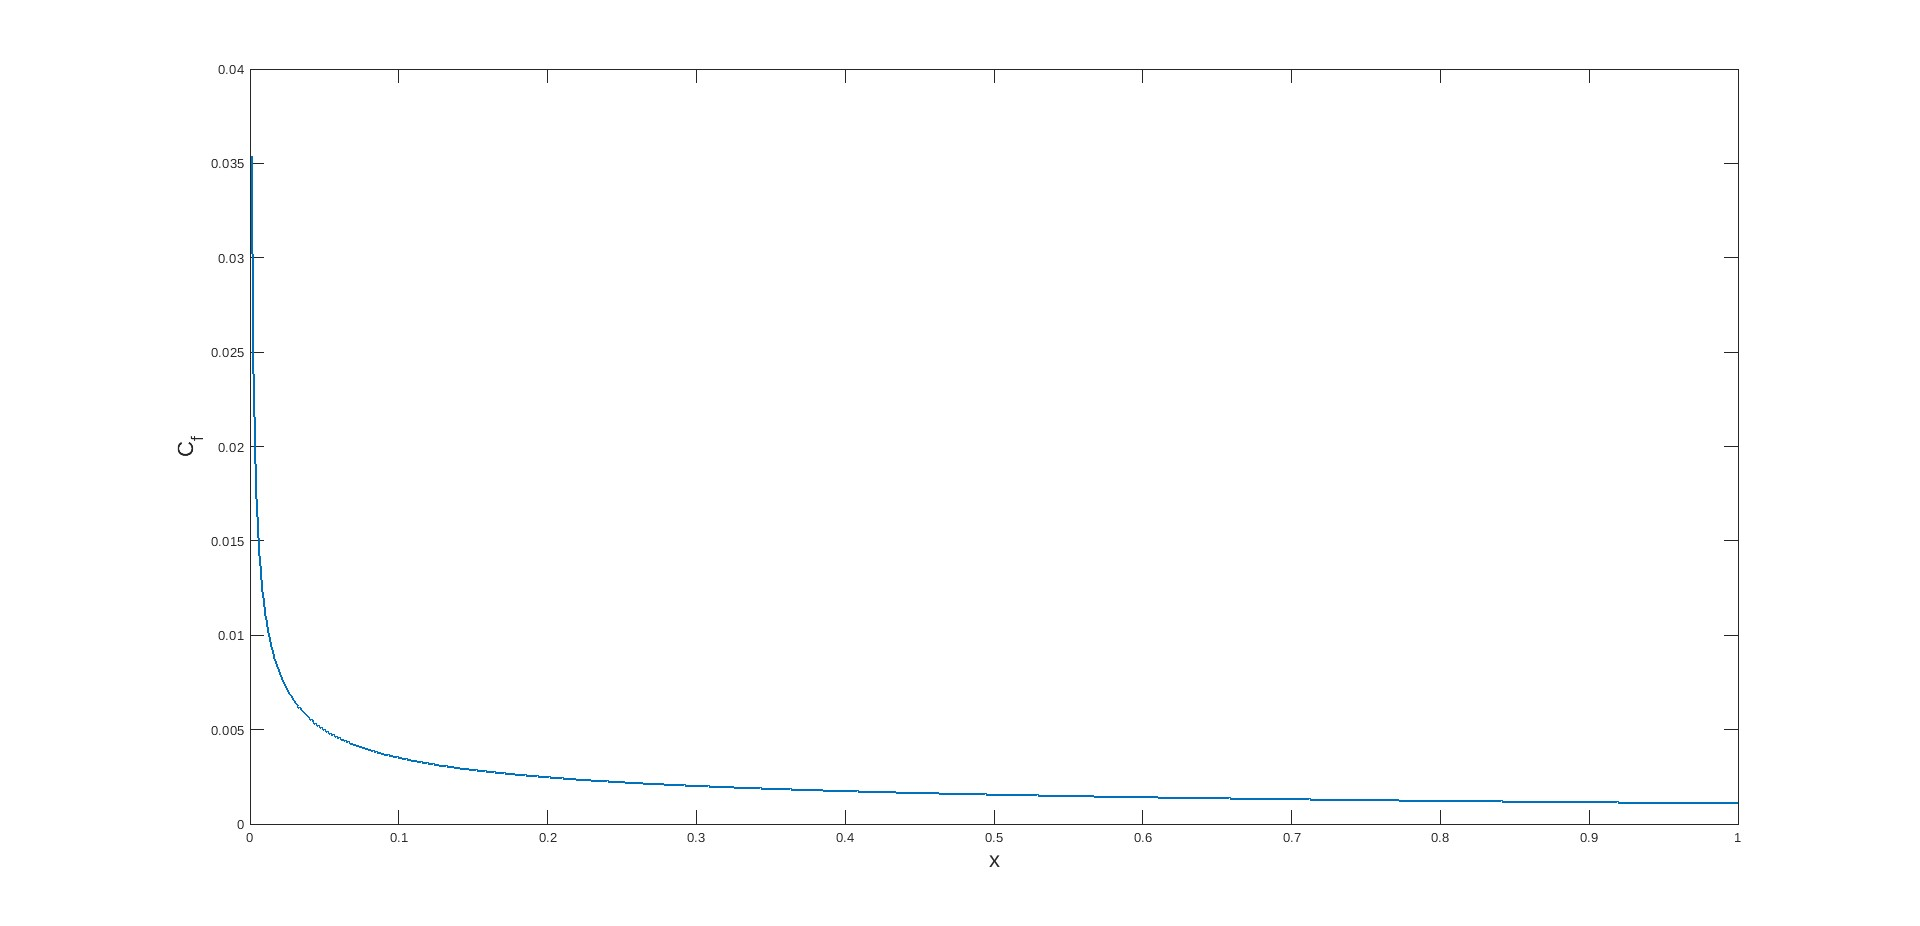
\includegraphics[width=\linewidth]{cf.jpg}
    \caption{ friction coefficient along the wall $C_f$ vs. $x$ (Code \ref{func:CF})}
    \label{fig:cf}
\end{figure}

\newpage
\chapter*{Acknowledgements}

This project was undertaken as part of the requirements for ENGR 6201: Fluid Mechanics, lectured by Professor Karimfazli at Concordia University, Montreal, Canada. The report was meticulously prepared using the \LaTeX\ typesetting language on the \href{https://www.overleaf.com/}{Overleaf} platform. The MATLAB\cite{MATLAB} R2022b Linux version was employed for code generation and visualization of graphs. Additionally, schematic diagrams were crafted using \href{https://app.diagrams.net/}{draw.io}

\nomenclature[a01]{$A$}{Area $(m^2)$}
\nomenclature[a02]{$C_D$}{Drag Coefficient $(-)$}
\nomenclature[a03]{$C_f$}{Friction Coefficient $(-)$}
\nomenclature[a04]{$F_D$}{Drag force$(N)$}
\nomenclature[a05]{$P$}{Pressure $(Pa)$}
\nomenclature[a06]{$t$}{time $(s)$}
\nomenclature[a07]{$U_e$}{ Free Stream velocity $(m/s)$}
\nomenclature[a08]{$u$}{ velocity component in $x$ direction $(m/s)$}
\nomenclature[a09]{$v$}{ velocity component in $y$ direction $(m/s)$}
\nomenclature[a10]{$x$}{spatial coordinates $(m)$}
\nomenclature[a11]{$y$}{spatial coordinates $(m)$}
\nomenclature[a12]{$\delta$}{thickness of boundary layer $(m)$}
\nomenclature[a13]{$\mu$}{Dynamic viscosity $(Pa.s)$}
\nomenclature[a14]{$\nu$}{Kinematic viscosity $(m^2/s)$}
\nomenclature[a15]{$\rho$}{density $(kg/m^3)$}
\nomenclature[a16]{$\tau$}{Shear Stress $(N/m^2)$}
\nomenclature[a17]{$\psi$}{Stream Function}

\printnomenclature
\bibliographystyle{ieeetr}
\bibliography{bib}
\newpage
\appendix

\chapter{Matlab Code}

\section{functions}

\subsection{Blasius O.D.E}
\label{func:bla}
\begin{lstlisting}[
frame=single,
numbers=left,
style=Matlab-Pyglike]
function dydt = blasius(eta, y)
       dy1dt = y(2);
       dy2dt = y(3);
       dy3dt = -0.5 * y(1) * y(3);
       dydt = [dy1dt; dy2dt; dy3dt];
\end{lstlisting}

\subsection{$\eta(x,y)$ function}
\label{func:eta}

The following function calculates the dimensionless variable $\eta$ as defined in Eq. \ref{eq:eta}.

\begin{lstlisting}[
frame=single,
numbers=left,
style=Matlab-Pyglike]
function eta_value = Eta_func(x,y,U_e, nu)
    nux = nu .* x;
    Unux = U_e .* (nux .^ -1);
    eta_value = y .* sqrt(Unux);
end
\end{lstlisting}

\subsection{finding appropriate $f''(\eta=0)$}
\label{func:G_find}

The following function is designed to determine the suitable value for $f''(\eta=0)$, which satisfies the desired boundary conditions. This function will be used by `shootingMethod` function.
\begin{lstlisting}[
frame=single,
numbers=left,
style=Matlab-Pyglike]
function res = G_find(G)
    [~,f] = ode78(@blasius,[0 10],[0;0;G]);
    res = f(end,2) -1;
end
\end{lstlisting}

\subsection{Shooting Method}
\label{{func:shoot}}

The following function is designed to determine the root of the given function to desired tolerance:
\begin{lstlisting}[
frame=single,
numbers=left,
style=Matlab-Pyglike]
function root = shootingMethod(inputFunction, initialGuess, tolerance)
    x0 = initialGuess;
    dx = 1e-6;
    maxIterations = 1000;
    for iteration = 1:maxIterations
        f = inputFunction(x0);
        dfdx = (inputFunction(x0 + dx) - f) / dx;
        x0 = x0 - f / dfdx;
        if abs(f) < tolerance
            root = x0;
            return;
        end
    end
end
\end{lstlisting}

\subsection{Shear Stress}
\label{func:tau}
The following function  calculates the shear stress using the provided parameters. This function is based on Eq.\ref{eq:tau}.

\begin{lstlisting}[
frame=single,
numbers=left,
style=Matlab-Pyglike]
function shear = tau(x,U_e,mu, rho,G)
    nu = mu /rho;
    g = sqrt(U_e ./ ( nu * x));
    shear = mu * U_e * g * G;
end
\end{lstlisting}

\subsection{Friction Coefficient}
\label{func:CF}
The following function  calculates the friction coefficient along the wall using the provided parameters. This function is based on Eq.\ref{eq:CF}.

\begin{lstlisting}[
frame=single,
numbers=left,
style=Matlab-Pyglike]
function Cf_value = Cf(x ,mu,rho, U_e,G)
    tau_value = tau(x, U_e, mu, rho, G);
    Cf_value = (2* tau_value) / (rho * U_e);
end
\end{lstlisting}

\subsection{Boundary Layer Thickness}
The following function computes the boundary layer thickness in the give $x$ based on Eq.\ref{eq:eta}.
\begin{lstlisting}[
frame=single,
numbers=left,
style=Matlab-Pyglike]
function value = thickness(x,U_e,nu)
    value = sqrt(nu * x / U_e);
end
\end{lstlisting}

\subsection{Analytical Solution}
\label{func:anal}
The following function represents Eq.\ref{eq:anal} in Matlab code:
\begin{lstlisting}[
frame=single,
numbers=left,
style=Matlab-Pyglike]
function fp = analyitical(eta,a,n)
    fp = (tanh((a*eta).^n)).^(1/n);
end
\end{lstlisting}

\section{Main Code}
\subsection{Cleaning and defining hyper-paramaters}

The following code serves the purpose of cleaning the workspace and setting up essential hyper-parameters and constant values for the subsequent numerical simulation.

\begin{lstlisting}[
frame=single,
numbers=left,
style=Matlab-Pyglike]
%% cleaing 
close all;clear;clc
format long


%% Setting hyperparameters and constant values
L = 1;
H = 0.02;

dy = 0.0001;
dx = 0.001;

x = 0.001:dx:L;
y = 0.001:dy:H;
\end{lstlisting}

If the $u$ velocity component along the $y$-axis at a specific $x$ is required, the following code can be used in place of lines 13 and 14 of the previous code:

\begin{lstlisting}[
frame=single,
numbers=left,
style=Matlab-Pyglike]
x= [0.05,0.1,0.15,0.2,0.25];
H = tickness(x,U_e,nu);
y = 0:H/5000:H*20;
\end{lstlisting}
\subsection{Compute $\eta$ values}
The following code is to generate the meshgird and compute $\eta$ values using function \ref{func:eta}. 
\begin{lstlisting}[
frame=single,
numbers=left,
style=Matlab-Pyglike]
%% Generating meshgrid and computing eta
[X,Y] = meshgrid(x,y);
eta = Eta_func(X,Y,U_e,nu);
\end{lstlisting}

\subsection{Finding the $f''(\eta=0)'$}
The following command finds the appropriate $f''(\eta=0)$ which satisfies the boundary conditions with root finding function 'shootingMethod'. The 'G\_find' function is defined in \ref{func:G_find}.

\begin{lstlisting}[
frame=single,
numbers=left,
style=Matlab-Pyglike]
tol = 0.00001;
G = shootingMethod(@G_find,1,tol)

\end{lstlisting}

\subsection{Solving the Blasius Equation}
Different Solutions generated by the following code, the 'blasius' and 'analytical' functions are defined by \ref{func:bla} and \ref{func:anal}, respectively :
\begin{lstlisting}[
frame=single,
numbers=left,
style=Matlab-Pyglike]
%% solivng with different methods
sol23 = ode23(@blasius,[0 10],[0;0;G]);
sol45 = ode45(@blasius,[0 10],[0;0;G]);
sol78 = ode78(@blasius,[0 10],[0;0;G]);
sol89 = ode89(@blasius,[0 10],[0;0;G]);

t = linspace(0,10,1000);

f23 = deval(sol23,t);
f45 = deval(sol45,t);
f78 = deval(sol78,t);
f89 = deval(sol89,t);

f_analytic = analyitical(t,G,3/2);
\end{lstlisting}

\subsection{Root Mean Square Error}
The following code is utilized to compute Root Mean Square Error defined by Eq.\ref{eq:rmse}:
\begin{lstlisting}[
frame=single,
numbers=left,
style=Matlab-Pyglike]
%% compute root mean squeres
RMSE23 = sqrt(mean((f23(2,:) - f_analytic).^2));
RMSE45 = sqrt(mean((f45(2,:) - f_analytic).^2));
RMSE78 = sqrt(mean((f78(2,:) - f_analytic).^2));
RMSE89 = sqrt(mean((f89(2,:) - f_analytic).^2));
\end{lstlisting}

\subsection{Finding $\eta_{max}$}
By varying 'criteria' in the followig code the table \ref{tab:eta_max} is generated:
\begin{lstlisting}[
frame=single,
numbers=left,
style=Matlab-Pyglike]
%% finding the eta_max
criteria = 0.000001;
index_eta_max = find(diff(f89(2,:))./f89(2,2:end)<criteria,1);
eta_max = t(index_eta_max);
\end{lstlisting}

\subsection{Computing $u$,$v$ velocity components}

To create a function from the solution of ODE78 to be able to predict new values if needed, 'interp1' Matlab was used. to increase the accuracy the solution was divided to two parts. the first par is in the range of $0<\eta<\eta_{max}$ which $f'(\eta)$ rises from $0$ to $1$ and the second part represents $\eta_{max} < \eta$ in which $f'(\eta)$ is approximately $1$.

\begin{lstlisting}[
frame=single,
numbers=left,
style=Matlab-Pyglike]
%% Computing u and v
fp1 = eta > eta_max;

F = f89(2,1:index_eta_max);
T = t(1:index_eta_max);

fp2 = zeros(size(eta,1), size(eta,2));
f = zeros(size(eta,1), size(eta,2));
for i=1:1:size(eta,2)
    fp2(:,i) = interp1(T,F,eta(:,i)) .* (eta(:,i) < eta_max);
    f(:,i) = interp1(T,F,eta(:,i));
end

fp1(isnan(fp1))=0;
fp2(isnan(fp2))=0;
f(isnan(f))=0;

fp = fp1 + fp2;

u = U_e .* fp;
v = nu .* thickness(x,U_e,nu) .* (eta .* fp - f);
\end{lstlisting}

\subsection{Shear Stress, Force and Drag Coefficient}

\begin{lstlisting}[
frame=single,
numbers=left,
style=Matlab-Pyglike]
%% shear stress
taus = tau(x,U_e,1.7*(10^-5),1.2,G);

fun = @(nx) tau(nx,U_e,1.7*(10^-5),1.2,G);

q = integral(fun,0.00,1);
C_D = q/(U_e^2 * rho)
\end{lstlisting}

\section{Plots}

\subsection{Contour of $\eta$ values}
\label{func:eta_val}
Contour of $\eta$ values with respect to $x$ and $y$
\begin{lstlisting}[
frame=single,
numbers=left,
style=Matlab-Pyglike]
%% ploting eta values
contourf(x,y,log10(eta),50,'edgecolor','none');

cb = colorbar('Ticks',[0,1,2,3,4],'TickLabels',{'0', '10^1','10^2','10^3','10^4'});

cb.Label.String = '\eta';
cb.Label.FontSize=18;

colormap turbo;
xlabel('x','FontSize',16);
ylabel('y','FontSize',16);

\end{lstlisting}

\subsection{Plot of $f'(\eta)$ and $f''(\eta)$}
\label{func:bla_sol}
\begin{lstlisting}[
frame=single,
numbers=left,
style=Matlab-Pyglike]
%% ploting f, fp

hold on
plot(t,f89(2,:),'-o','MarkerIndices',1:20:length(f89(2,:)),'LineWidth',2,'DisplayName','f''(\eta)');
plot(t,f89(3,:),'-*','MarkerIndices',1:20:length(f89(3,:)),'LineWidth',2,'DisplayName','f''''(\eta)');

xlabel('\eta','FontSize',16);
ylabel('F','FontSize',16);

lgd = legend();
lgd.FontSize = 18;
\end{lstlisting}

\subsection{Contour of $u$ velocity component}
\label{func:u}
\begin{lstlisting}[
frame=single,
numbers=left,
style=Matlab-Pyglike]
%% Plotting u
hold on
contourf(x,y,u,50,'edgecolor','none');

cb = colorbar;
cb.Label.String = 'u';
cb.Label.FontSize=18;

colormap spring;

xlabel('x','FontSize',16);
ylabel('y','FontSize',16);
\end{lstlisting}

\subsection{Contour of $v$ velocity component}
\label{func:v}
\begin{lstlisting}[
frame=single,
numbers=left,
style=Matlab-Pyglike]
%% Plotting v
hold on
contourf(x,y,v,50,'edgecolor','none');

cb = colorbar;
cb.Label.String = 'v';
cb.Label.FontSize=18;

colormap spring;

xlabel('x','FontSize',16);
ylabel('y','FontSize',16);
\end{lstlisting}

\subsection{Plot Shear Stress on the plate}
\label{func:tau}
\begin{lstlisting}[
frame=single,
numbers=left,
style=Matlab-Pyglike]
%% shear stress
taus = tau(x,U_e,1.7*(10^-5),1.2,G);

plot(x,taus,'LineWidth',2);

xlabel('x','FontSize',16);
ylabel('\tau','FontSize',16);
\end{lstlisting}

\subsection{Plot $u$ velocity at specific positions}
\label{func:xspec}
Plotting $u$ velocity component along $y$-axis at specific $x$ positions
\begin{lstlisting}[
frame=single,
numbers=left,
style=Matlab-Pyglike]
plot(u,y,'LineWidth',2)
legend('x = 0.05 m','x = 0.10 m', 'x = 0.15 m', 'x = 0.20 m','x = 0.25 m','FontSize',16)
xlabel('U(m/s)',"FontSize",18);
ylabel("y(m)","FontSize",18);
\end{lstlisting}

\subsection{Plotting $f'(\eta_{max})$ vs. $f''(0)$}
\label{func:G_find}
\begin{lstlisting}[
frame=single,
numbers=left,
style=Matlab-Pyglike]
x = linspace(0,1,100);
Y = zeros(1,100);

for i=1:size(x,2)
    Y(1,i) = G_find(x(i))+ 1;
end

hold on
plot(x,Y,'LineWidth',2);
plot(0.332057334445899,1,'r*')

xline(0.332057334445899,'--');
yline(1,'--')

xlabel("initial f''''(\eta=0)");
ylabel("\eta_{final}")
\end{lstlisting}

\subsection{Plotting numerical solution errors}
\label{func:errors}
\begin{lstlisting}[
frame=single,
numbers=left,
style=Matlab-Pyglike]
%% ploting errors
hold on
plot(t,(f23(2,:)-f_analytic),'r-','DisplayName','ODE23','LineWidth',2);
plot(t,(f45(2,:)-f_analytic),'y-','DisplayName','ODE45','LineWidth',2);
plot(t,(f78(2,:)-f_analytic),'g-','DisplayName','ODE78','LineWidth',2);
plot(t,(f89(2,:)-f_analytic),'b-','DisplayName','ODE89','LineWidth',2);

lgd = legend();
lgd.FontSize = 18;

%title("Numerical methods error in comparison to Analyitcal Solution",'FontSize',18)
xlabel('\eta','FontSize',16);
ylabel('error','FontSize',16);
\end{lstlisting}
\end{document}
